\scanpage{5}
\[
\operatorname{réal}(S,A,R)\lhook\joinrel\longrightarrow E
\]
telle que l'image d'un arc soit un segment.

\uline{Prop} Pour qu'un graphe fini admette une réalisation géom. rectiligne, (dans un vectoriel convenable sur $\mathbb{R}$) il f et s qu'il \deleted{\unsure{a|est}} soit strict -- et alors il admet une réalisation rectiligne dans $\mathbb{R}^{3}$. De façon précise, si $S\hookrightarrow\deleted{\unsure{\mathbb{R}^{3}|R^{3}}}E$ \inserted{$(\simeq\mathbb{R}^{3},\ \unsure{v.a.|v.ex.})$} est une immersion telle que
\figure{\begin{tikzpicture}[x=.025cm,y=.025cm]
\draw[line width=.7pt] (0,0)--(31,34);
\draw[line width=.3pt] (34,38)--(60,66);
\draw (0,0) circle (1.5);
\fill (31,34) circle (1.45);
\fill (60,66) circle (1.2);
\end{tikzpicture}}
\[
\forall x,y\in S\quad x\ne y,\quad \text{on ait}\quad
\deleted{\unsure{\{|\exists}}
\underbrace{\overline{x,y}}_{\substack{\text{segm}\\\text{joignant}\\x\ \text{à}\ y}}\cap S=\{x,y\},
\]
\inserted{(i.e. trois points \inserted{distincts} jamais alignés)}
\inserted{et $\forall x,y,z,t$ distincts, $(\overline{x,y})\cap(\overline{z,t})=\varnothing$}

$\exists 1$ réalis géom. rectiligne $\unsure{\operatorname{réll}|\operatorname{réel}|\operatorname{réal}}(S,A,R)\lhook\joinrel-E$ qui f \unsure{prolonge|prolonge\textsuperscript{?}}\ldots

Graphe connexe $=$ réal. géom connexe $=$ qui n'est pas \deleted{\unsure{réunion}} ``somme'' de deux autres graphes $\ne\varnothing$

\uline{NB} Tout graphe est de façon unique réunion de graphes connexes \inserted{et disjoints}

[ graphe somme : $S\amalg S',\quad A\amalg A',\quad R\amalg R'\ \ldots$ ]

% A curved arrow in the left margin leads from NB to the next heading.
\margin{\figure{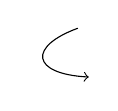
\begin{tikzpicture}[baseline=-.5ex,x=1cm,y=1cm]\draw[->] (.48,.62) .. controls (-.15,.39) and (-.12,.04) .. (.62,0);\end{tikzpicture}}}
Graphe \inserted{multi}polygonal \inserted{(ou \uline{contour} (combinatoire))}
\[
\bigl[\quad\forall s\in S,\quad\operatorname{card}R\{s\}=2\quad\bigr]
\]

Dualité des \deleted{graphes polygonaux} contours (combinatoires).

\deleted{\unsure{donq|donc}} les composantes \inserted{\unsure{conn.|connexes}} d'un \deleted{graphe polygonal}\inserted{contour} sont \deleted{polygonales.} des contours.

Classification des \deleted{graphes polygonaux}\inserted{contours} conn. $\ne\varnothing$

\uline{Prop} Un \deleted{graphe polyg.}\inserted{contour} connexe \inserted{$\ne\varnothing$} est connu à isom. près quand on connait $\operatorname{card}S$ ($=\operatorname{card}A$), qui est n'importe quel cardinal \deleted{fini ou infini}
\[
2\le c\le\aleph_{0}
\]
(strict \unsure{ssi|sss} $c\ne2$ i.e. $c\geqslant3$)
% archive sheet number: 4
